\section{Présentation du Challenge MOBILEX}
Comme mentionné précédemment, le Challenge MOBILEX* vise à accélérer la recherche et à faire mûrir technologiquement le domaine de la navigation autonome des véhicules en Environnement complexe*.\\\\
\indent Pour ce faire, les organisateurs ont lancé un appel à projet auquel pouvaient candidater des consortiums composés d'au moins un acteur industriel et d'un acteur de la recherche française. L'objectif était de rendre un véhicule imposé autonome pour des cas de situations donnés et de proposer des fonctionnalités/aides facilitants le contrôle par un téléopérateur.\\\\
\indent À l'issue de l'appel à projets, sept consortiums ont été retenus comme ci-après (Figure \ref{fig3}) :

\begin{figure}[H] % Utilisez [H] au lieu de [htb]
  \centering % Utilisez \centering au lieu de \makebox
  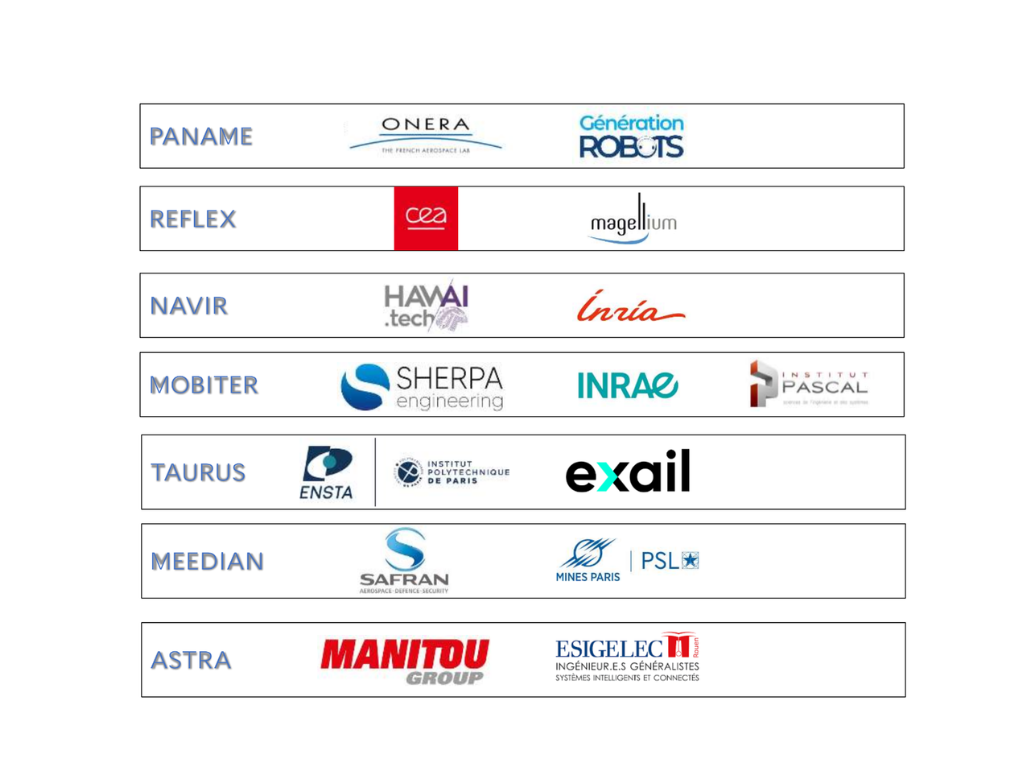
\includegraphics[trim={0.0cm 1cm 0.0cm 2cm}, clip, width=1.05\linewidth]{Corps_rapport/Liste_consortiums.png}
  \caption{Liste des équipes du challenge}
  \label{fig3}
\end{figure}

\subsection{Le consortium MOBITER}
Pour répondre au mieux aux ambitions du Challenge MOBILEX*, SHERPA Engineering s'est associée avec ses partenaires académiques INRAE et Institut Pascal, avec lesquels elle collabore régulièrement grâce à une proximité géographique, un laboratoire qui était jusqu'à récemment commun pour SHERPA Engineering et l'Institut Pascal, et des propositions régulières de thèses CIFRE.\\\\
\indent Cette proximité permet de répartir aisément les tâches à réaliser en fonction de l'expertise de chacun et de faciliter la communication entre les différents acteurs, notamment grâce à un canal Teams sur lequel sont partagés les avancées et différents documents et où une réunion hebdomadaire a lieu, permettant de présenter le travail de chacun et de planifier les tests sur le terrain. Les apports de chaque partie sont les suivants :

\subsubsection{SHERPA Engineering}
SHERPA Engineering, coordinatrice du projet, réalise, sur la base d'un existant, la mise en place de la base hardware du projet en l'adaptant pour répondre aux exigences du challenge. Elle réalise les tâches d'ingénierie du projet et a la charge d'une partie de l'algorithmie liée à la perception et à la planification.

\subsubsection{INRAE}
L'INRAE apporte son expérience dans la robotique agricole, notamment sur les nouvelles lois de commande, et est responsable de l'expérimentation grâce à l'utilisation de ses sites à Aubière (Puy-de-Dôme) et Montoldre (Allier).

\subsubsection{Institut Pascal}
L'Institut Pascal fournit des conseils sur le développement scientifique (fusion de données, traversabilité, gestion des risques, planification) qui sont mis en application par une ressource interne.



\subsection{Les attendus du challenge}
\subsubsection{Organisation générale}
Le Challenge Mobilex* est organisé par les acteurs suivants (Figure \ref{fig4}) :

\begin{figure}[H] % Utilisez [H] au lieu de [htb]
  \centering % Utilisez \centering au lieu de \makebox
  
\includegraphics[width=1.05\linewidth]{Corps_rapport/Organisateurs_challenge_mobilex.png}
  \caption{Organisateur du challenge Mobilex}
  \label{fig4}
\end{figure}

\indent Il se déroule sur trois années et est composé de trois défis de difficulté croissante, à savoir un défi par annnée. Les modalités de ces défis ne sont communiquées aux équipes qu'au début de chaque défi \cite{anr2023mobilex}. À la fin de chaque année, toutes les équipes sont convoquées sur un site de la DGA pour y être évaluées sur leurs propositions en réponse aux situations rencontrées lors du défi.\\\\
\indent L'organisation de chaque défi se déroule comme suit (Figure \ref{fig5}) :

\begin{figure}[H] % Utilisez [H] au lieu de [htb]
  \centering % Utilisez \centering au lieu de \makebox
  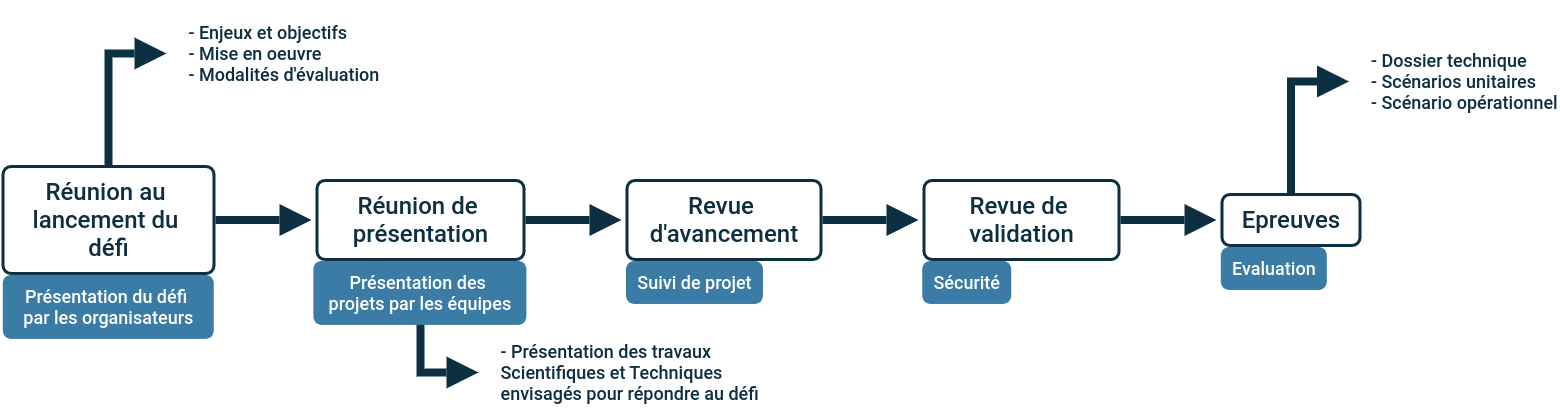
\includegraphics[width=1.05\linewidth]{Corps_rapport/timeline_defi.png}
  \caption{Déroulement d'un défi}
  \label{fig5}
\end{figure}

\subsubsection{Fonctions attendues}
Pour chaque défi, une liste de nouvelles fonctions attendues est donnée. Les fonctions demandées lors des précédents défis doivent également fonctionner lors des scénarios du défi en cours (sauf indication contraire de la DGA). Ces fonctions peuvent être classées selon deux modes de fonctionnement : le mode pilote automatique et le mode téléopération assistée.

\paragraph{Mode pilote automatique}
Pour le premier défi, les fonctions attendues étaient les suivantes :\\
\begin{itemize}
\renewcommand{\labelitemi}{$\bullet$}
    \item Détection et gestion locale des obstacles positifs franchissables et non franchissables.
    \item Détection et gestion locale des bas-côtés positifs.
    \item Fonction rejeu de trajectoire.
    \item Fonction retour sur trace.
    \item Évitement de zones d'exclusion, d'interdiction et passage par des points de passage imposés.\\
\end{itemize}

Le second défi a quant à lui demandé l'ajout des fonctions suivantes :\\
\begin{itemize}
\renewcommand{\labelitemi}{$\bullet$}
    \item Détection et gestion locale des obstacles négatifs franchissables et non franchissables.
    \item Détection et gestion locale des obstacles transparents/réflichissants.
    \item Détection et gestion locale des bas-côtés négatifs.
    \item Prise en compte des pentes positives et négatives.
    \item Détection et gestion locale des dévers.
    \item Gestion des situations dégradées (pannes capteurs, perte de communication avec le poste de téléoperation, ...).\\
\end{itemize}

Lors du troisième et dernier défi, les équipes se sont vu supprimer certaines fonctions imposées au cours des précédents défis, à savoir :\\
\begin{itemize}
\renewcommand{\labelitemi}{$\bullet$}
    \item Le rejeu de trajectoire et le retour sur trace.
    \item Détection et gestion locale des obstacles transparents/réflichissants.
    \item Détection et gestion locale des obstacles à bascules.
    \item Le changement artificiel de gabarit.
    \item Gestion des pannes capteurs. \\
\end{itemize}

Et se sont vu rajouter les nouvelles fonctions suivantes :\\
\begin{itemize}
\renewcommand{\labelitemi}{$\bullet$}
    \item Gestion des pentes et dévers avec obstacles franchissables ou non.
    \item Gestion de la végétation et des flaques d'eau.
    \item Suivi de bas-côtés (positif et négatif) avec gestion d'obstacles sur la trajectoire.
    \item Gestion des situations dégradées (perte des donnés gnss, perte de communication avec le poste de téléoperation, ...).
\end{itemize}


\paragraph{Mode téléopération assistée}
Pour le premier défi, une IHM fonctionnant sur un PC déporté a été demandée pour, au minimum, pouvoir choisir le mode de pilotage, renvoyer les commandes réalisées par le téléopérateur lors d'un pilotage manuel et fournir un retour vidéo annoté. Ce retour vidéo doit contenir des informations concernant la compréhension de l'environnement établie par la brique logicielle de l'équipe ainsi que les indications de direction pour gérer la trajectoire.\\\\
\indent Lors du défi 2, un sous-mode \textit{Safety First} en téléopération assistée a été demandé. Ce mode vise à préserver l'intégrité du robot en imposant le respect des contraintes de navigation données par les organisateurs, en reprenant temporairement le contrôle du véhicule en cas de danger. Ce sous-mode doit être activable ou désactivable à tout moment depuis l'IHM.

\subsubsection{Contraintes de navigation à intégrer lors du développement}

\paragraph{Détection et gestion des obstacles}
En premier lieu, la navigabilité du véhicule repose sur la classification géométrique des obstacles rencontrés sur le terrain. Tout obstacle d'une hauteur ou d'une profondeur supérieure à 30~cm par rapport au sol est considéré comme non franchissable et impose un contournement. Le franchissement d'obstacles d'amplitude intermédiaire (entre 5 et 30~cm) est quant à lui conditionné par des limitations de vitesse strictes, nécessitant parfois un arrêt préalable (Figure~\ref{fig6}).

\begin{figure}[h!]
\centering
\begin{tabular}{|>{\columncolor{blue!30}}c|c|c|c|}
\hline
\rowcolor{blue!30} & avec arrêt & $<5$ km/h & $>5$ km/h \\
\hline
$<5$ cm & \textcolor{green!70!black}{Franchissable} & \textcolor{green!70!black}{Franchissable} & \textcolor{green!70!black}{Franchissable} \\
\hline
entre 5 cm et 15 cm & \textcolor{green!70!black}{Franchissable} & \textcolor{green!70!black}{Franchissable} & \textcolor{red}{Non franchissable} \\
\hline
entre 15 cm et 30 cm & \textcolor{green!70!black}{Franchissable} & \textcolor{red}{Non franchissable} & \textcolor{red}{Non franchissable} \\
\hline
$>30$ cm & \textcolor{red}{Non franchissable} & \textcolor{red}{Non franchissable} & \textcolor{red}{Non franchissable} \\
\hline
\end{tabular}
\caption{Gestion des obstacles en fonction de leur hauteur/profondeur et de la vitesse du robot}
\label{fig6}
\end{figure}

\paragraph{Détection et gestion des bas-côtés}
Au-delà des obstacles isolés, cette logique de franchissabilité s'applique directement à la détection continue de l'environnement périphérique. Ainsi, les bas-côtés (haies, murs, fossés, barrières, lisières) d'une hauteur supérieure à 30~cm (positive ou négative) doivent être détectés en permanence, quel que soit le mode de pilotage. La fonction de suivi de bas-côté impose au robot de maintenir une distance latérale consigne tout en adaptant dynamiquement sa trajectoire face aux obstacles (franchissables ou non) s'interposant sur son passage.

\paragraph{Détection et gestion des pentes et dévers avec obstacles}
Aux contraintes dimensionnelles des obstacles et des bas-côtés s'ajoutent les contraintes topologiques du relief. Les pentes (inclinaisons longitudinales dans l'axe de progression) et les dévers (inclinaisons transversales) supérieurs à 20° sont considérés comme hors du domaine de franchissabilité et doivent être détectés en continu. Lorsque des obstacles se superposent à ces pentes ou dévers, les règles d'infranchissabilité et d'adaptation de la vitesse sont combinées selon la logique récapitulée en Figure~\ref{fig7}.

\begin{figure}[H]
  \centering
  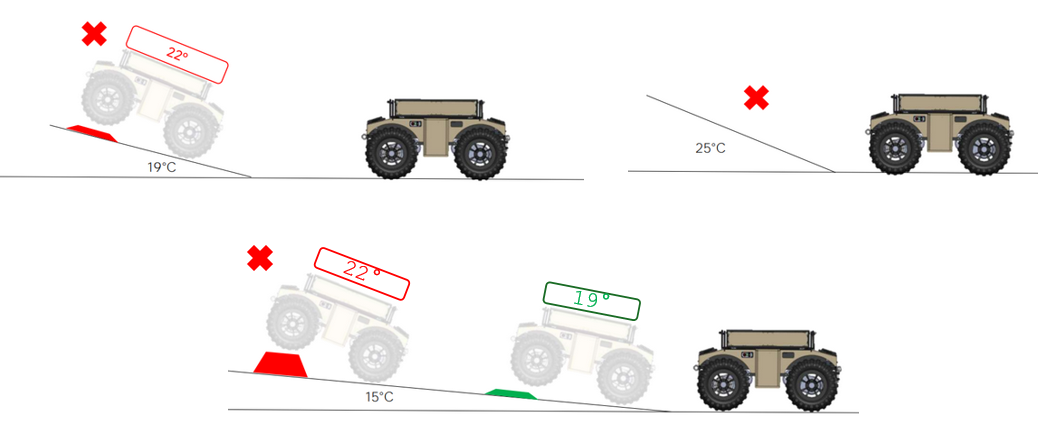
\includegraphics[width=1.05\linewidth]{Corps_rapport/Gestion_pentes.png}
  \caption{Gestion des pentes et dévers avec obstacles}
  \label{fig7}
\end{figure}

\paragraph{Gestion des situations dégradées}
Outre les contraintes physiques du terrain, le système doit garantir sa robustesse face aux perturbations environnementales et opérationnelles. Alors que le Défi~2 mettait l'accent sur la résistance aux intempéries (pluie, brouillard, fumée), le Défi~3 éprouve la capacité de la Brique MOBILEX* à maintenir l'ensemble de ses fonctions nominales en cas de couverture GNSS dégradée ou de perte de communication avec la station de contrôle débarquée.

\paragraph{Gestion des pannes capteurs}
Dans cette même optique de résilience, la brique logicielle doit tolérer des pannes matérielles transitoires (pannes brèves $< 10\text{~s}$ ou prolongées $< 2\text{~min}$) affectant individuellement le GPS, la caméra ou le LiDAR*. Bien que l'évaluation formelle de cette injection de pannes ne soit plus reconduite lors du Défi~3, cette exigence d'architecture demeure un pilier de la conception logicielle.

\paragraph{Points de passage imposés}
En complément de l'évitement d'obstacles et du suivi du relief, la trajectoire du robot est encadrée par des consignes de mission strictes. L'IHM doit permettre au téléopérateur de renseigner des points de passage imposés par les organisateurs. Le robot a pour obligation d'atteindre chacun de ces points selon l'ordre établi. Leurs coordonnées géographiques sont transmises sous forme de points cartésiens (projection UTM 31 dans le système géodésique WGS 84) avec une précision décimétrique.

\paragraph{Rejeu de trajectoire}
Sur la base de ces points de passage et des parcours enregistrés, le système propose des fonctionnalités avancées de renavigation. La Brique MOBILEX* doit pouvoir enregistrer et rejouer en autonomie n'importe quelle trajectoire préalable, quel que soit le mode de pilotage initial. Ce rejeu nécessite au préalable le repositionnement du robot au point de départ et doit adapter la trajectoire enregistrée en temps réel en cas d'apparition ou de modification d'obstacles. De plus, une option d'optimisation temporelle permet de réduire la durée de parcours tout en garantissant le franchissement ordonné des points de passage imposés.

\paragraph{Retour sur traces}
Répondant à une problématique complémentaire au rejeu, le retour sur traces permet au robot de regagner de manière autonome son point de départ (ou un point intermédiaire spécifié) en reprenant en sens inverse la trajectoire exactement parcourue à l'aller. Cette fonction, susceptible d'être déclenchée dans un contexte d'urgence, adapte sa planification face aux nouveaux obstacles et peut déroger aux limitations de vitesse nominales. Elle offre la flexibilité d'être exécutée en marche avant comme en marche arrière, avec changement de sens dynamique.

\paragraph{Zones d'exclusion}
Enfin, l'ensemble des algorithmes de planification de trajectoire (qu'il s'agisse du suivi de lisière, du rejeu ou du retour sur traces) doit intégrer des contraintes d'espace strictes définies par l'organisation. Les zones d'exclusion sont des polygones géographiques (coordonnées UTM 31) représentant des emprises interdites, pas nécessairement matérialisées sur le terrain. Tout franchissement de ces zones, tout comme la prise en compte erronée d'une zone virtuelle inexistante entraîne des pénalités au classement.

\paragraph{Zones d'interdiction}
Distinctes des zones d'exclusion par leur niveau de criticité, les zones d'interdiction constituent des enveloppes de sécurité absolue. Également définies sous forme de polygones géographiques (coordonnées UTM 31) virtuels, leur moindre chevauchement déclenche immédiatement un arrêt d'urgence du véhicule ainsi qu'une pénalité lourde, primant sur toutes les autres consignes de navigation.

\subsubsection{Évaluation des développements pour le défi en cours.}
L'évaluation des développements se fait à chaque défi et comporte trois notes : une note liée à la revue de validation, une note liée à la soumission du dossier scientifique et technique et une note liée aux épreuves. Elles visent à démontrer les capacités de développement de l'équipe et les performances du système développé.\\

\indent Lors de la journée d'épreuves sur un site de la DGA, les robots des équipes doivent accomplir une suite de scénarios donnés dans le règlement particulier du défi permettant d'évaluer des fonctions seules ou un ensemble de fonctions. Les équipes sont notées sur la bonne prise en compte de l'ensemble des contraintes fournies par les organisateurs et le bon fonctionnement des fonctions avec des critères de précision et/ou de rapidité.


\subsection{Présentation du robot BARAKUDA et des équipements embarqués}

\subsubsection{Plateforme robotique BARAKUDA}
Afin d'assurer la cohérence des évaluations entre les candidats, la DGA a fourni à chaque équipe le robot tout-terrain BARAKUDA, conçu par la société SHARK ROBOTICS (Figure~\ref{fig8}).

\begin{figure}[H]
  \centering
  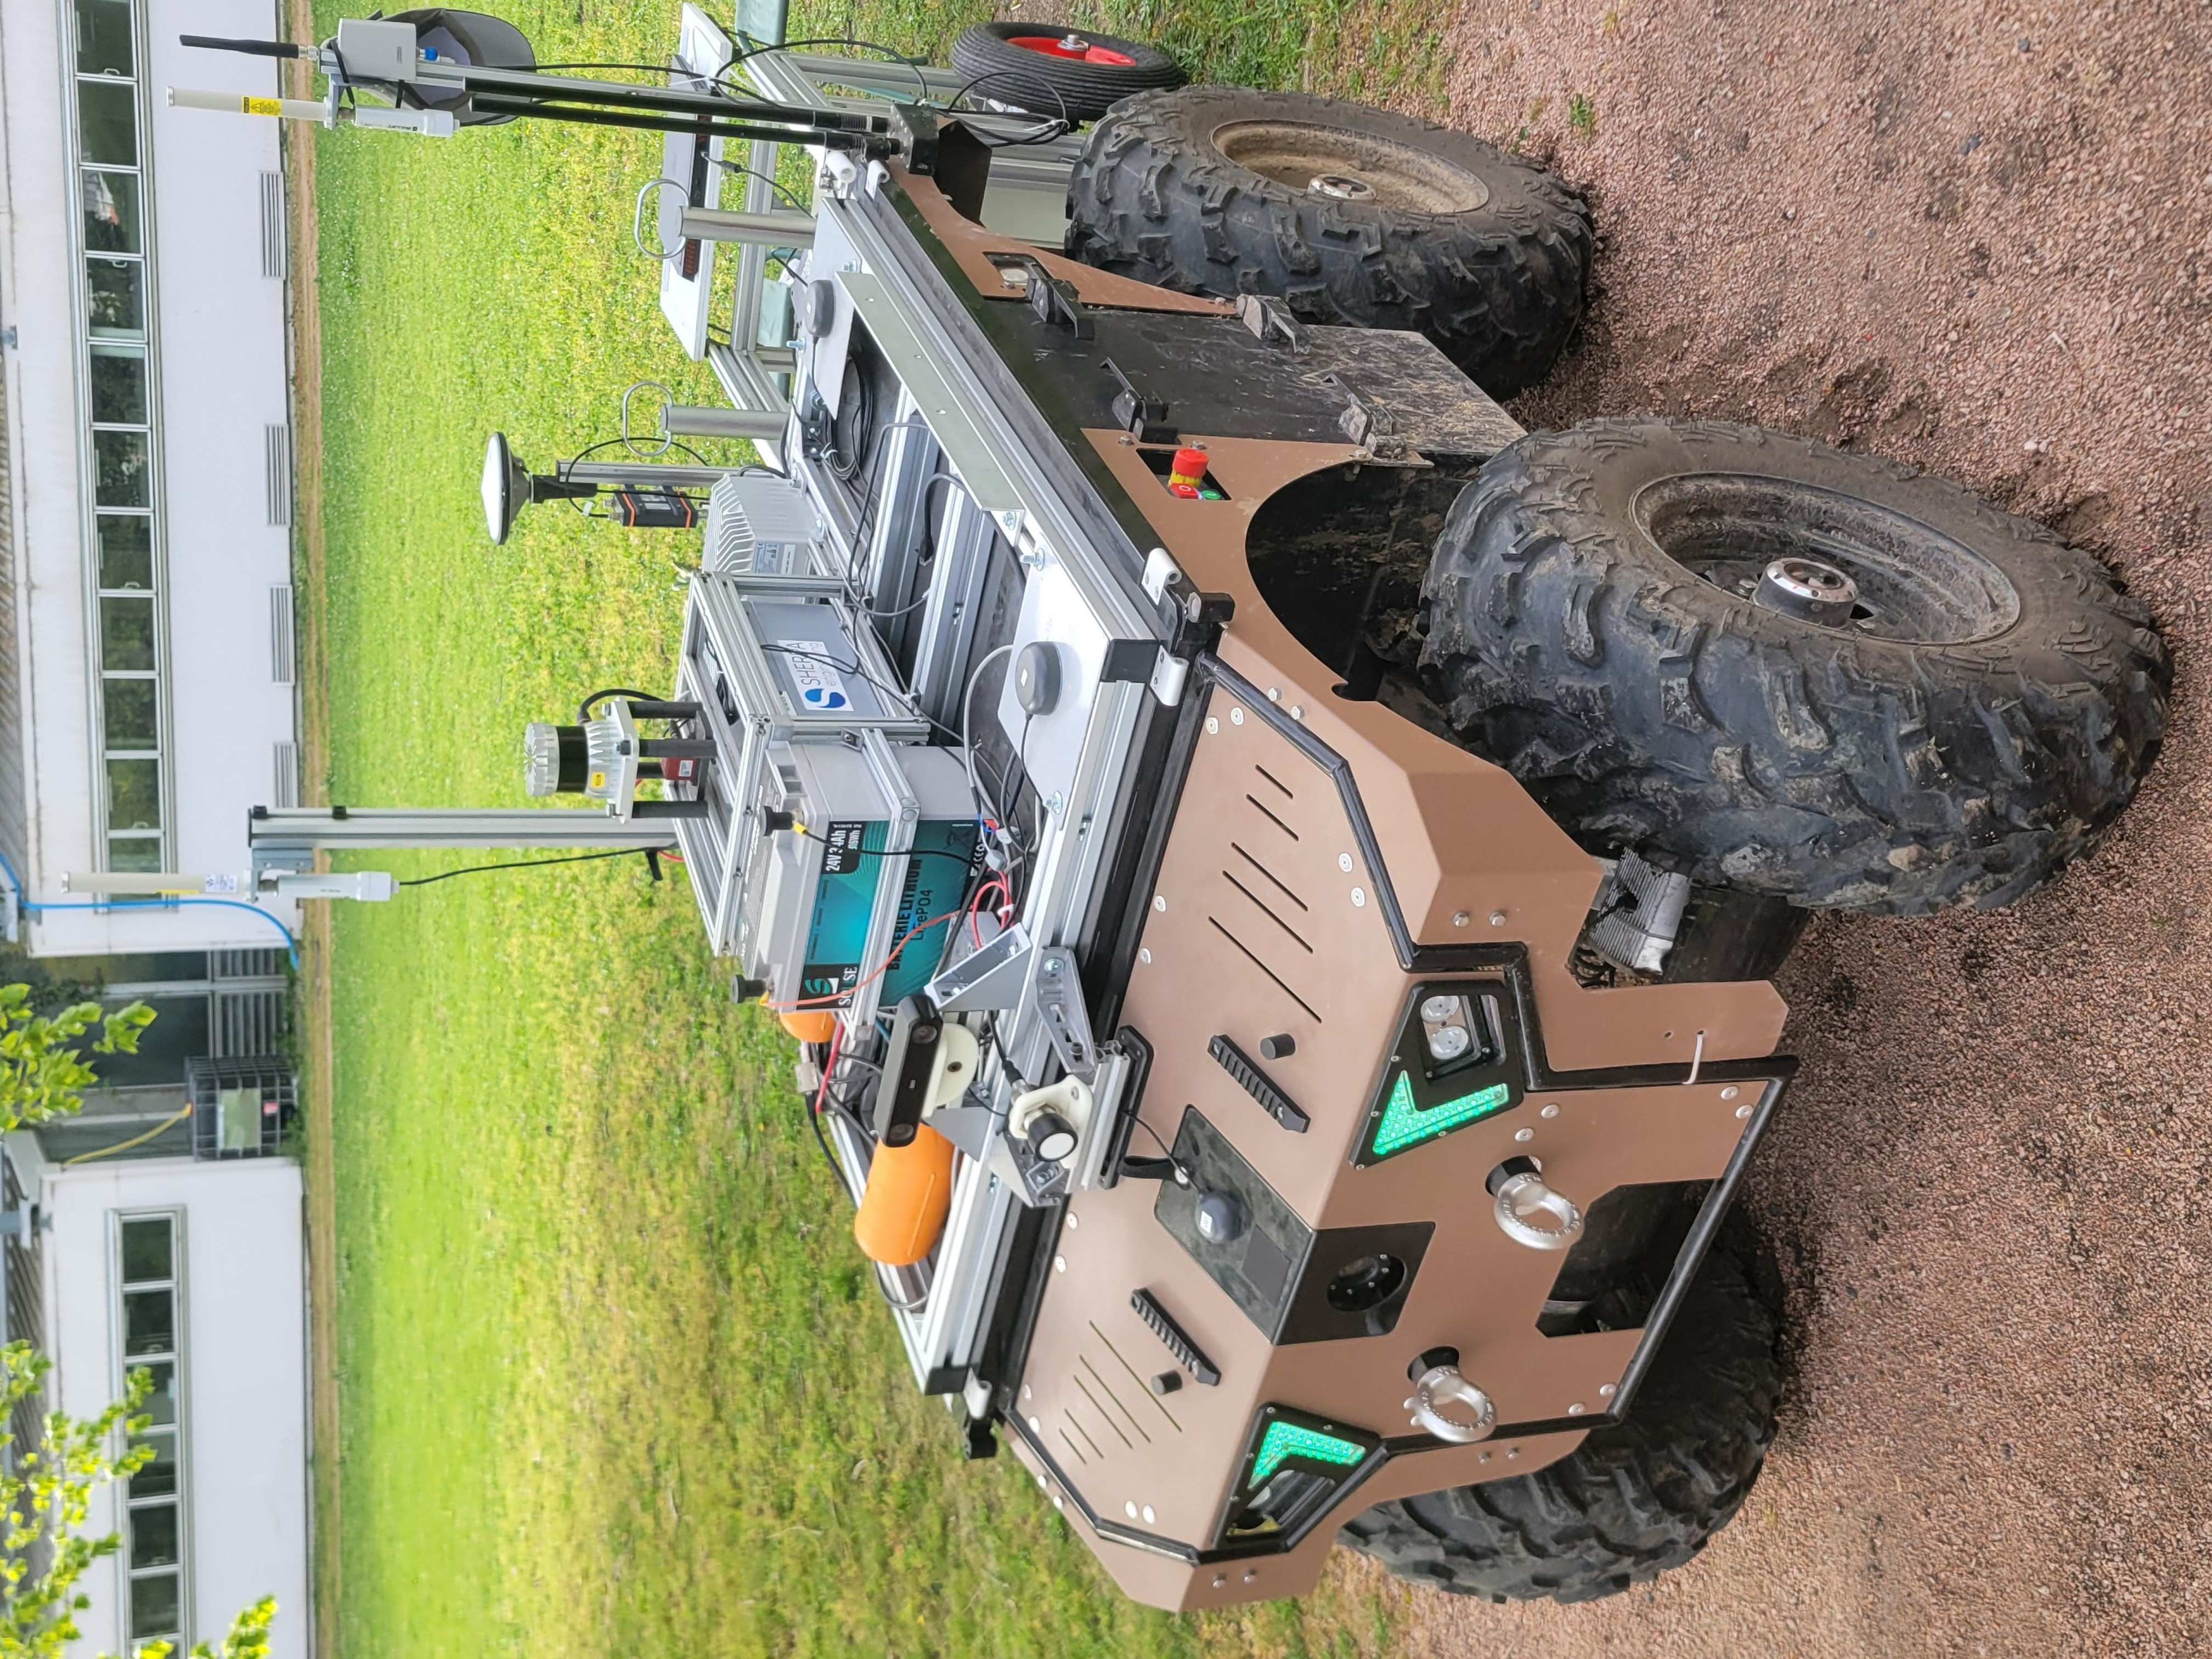
\includegraphics[width=0.5\linewidth, angle=-90]{Corps_rapport/barakuda.jpg}
  \caption{Plateforme mobile BARAKUDA (SHARK ROBOTICS)}
  \label{fig8}
\end{figure}

Il s'agit d'une plateforme chenillée à quatre roues motorisées non directionnelles d'une masse à vide de 500~kg, téléopérable jusqu'à une portée de 500 mètres en champ libre à l'aide de sa radiocommande d'origine. Capable de transporter une charge utile maximale de 500~kg, la plateforme atteint une vitesse de pointe de 20~km/h, franchit des obstacles d'une hauteur maximale de 30~cm et évolue sur des pentes jusqu'à 40° ainsi que des dévers jusqu'à 35°. En conditions opérationnelles, son autonomie atteint jusqu'à 10 heures.\\\\
\indent L'interface de communication entre le calculateur de bord et la Brique MOBILEX* s'appuie sur le protocole UDP (User Datagram Protocol). Ce choix garantit un traitement à très faible latence au détriment du contrôle d'acquittement, privilégiant ainsi l'actualité des données rafraîchies à haute fréquence. L'échange de données s'effectue via des trames structurées permettant d'envoyer les consignes de vitesse (linéaire et angulaire) et de collecter, par requêtes de type \texttt{GET}, l'état de santé du robot (vitesse et puissance moteur de chaque roue, inclinaisons attitude/cap, niveau de batterie et températures).

\subsubsection{Suite sensorielle et architecture matérielle ajoutées par le consortium}
Bien qu'il soit interdit de modifier la structure mécanique du robot, les équipes sont libres d'embarquer des équipements matériels dans la limite de la charge utile et du gabarit imposés. Le consortium MOBITER a ainsi équipé le robot avec les composants décrits ci-après (Figure~\ref{fig9}) :

\begin{figure}[H]
  \centering
  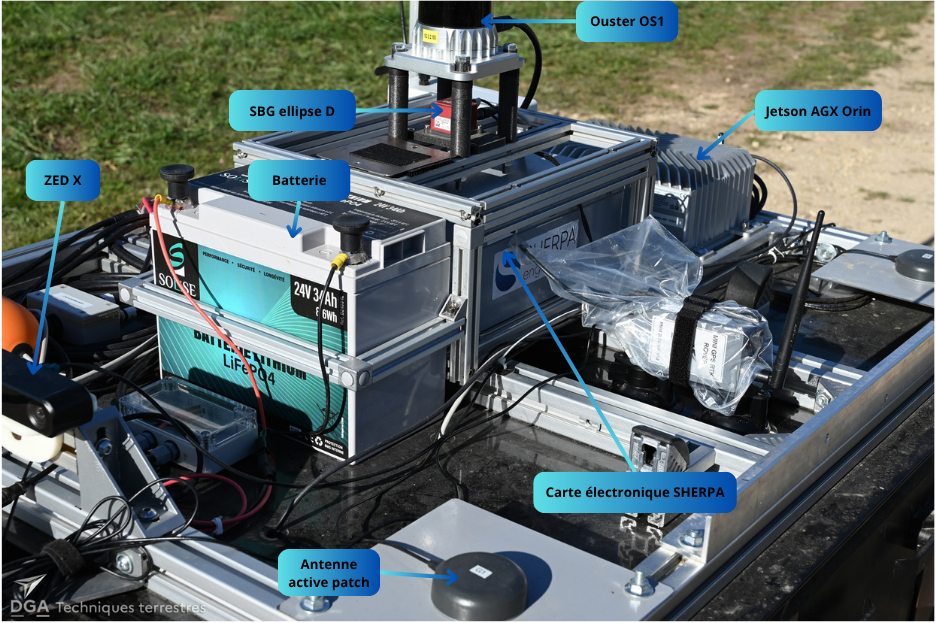
\includegraphics[width=0.7\linewidth]{Corps_rapport/Plateau_hardware.png}
  \caption{Implantation du plateau capteurs et des calculateurs embarqués}
  \label{fig9}
\end{figure}

\paragraph{Calculateur industriel Syslogic RML A4AGX}
%Afin d'absorber la charge de calcul engendrée par les nouvelles algorithmiques de perception et de planification, l'ancien calculateur Syslogic RML A3 a été remplacé par le modèle RML A4AGX. 
Ce calculateur industriel renforcé, à dissipation thermique passive, intègre un System-on-Module (SoM) NVIDIA Jetson AGX Orin. Il s'appuie sur un processeur ARM Cortex-A78AE à 12 cœurs (2,2~GHz), un GPU NVIDIA Ampere de 2048 cœurs CUDA, 64~Go de RAM LPDDR5 et des accélérateurs d'inférence deep learning NVIDIA DLA. Il dispose en outre de 6 contrôleurs Gigabit Ethernet indépendants et de 2 ports USB 3.1. Un SSD NVMe PCIe de 2~To a été ajouté en interne pour l'enregistrement à haute fréquence des données de logs (\emph{rosbags}). Ce composant a été retenu pour son excellente efficacité énergétique (ratio performance/Watt) et ses capacités de calcul parallèle adaptées à des applications robotiques et embarquées exigeantes.

\paragraph{Système de navigation inertielle (INS) SBG Ellipse-D}
Positionné au centre géométrique du plateau capteurs, ce système de navigation inertielle permet d'estimer en temps réel la pose 3D (position et orientation) ainsi que les vitesses linéaires et angulaires du robot. Il intègre une centrale inertielle (IMU) triaxiale étalonnée et compensée en température, couplée à un récepteur GNSS RTK double antenne permettant une estimation précise du cap même à l'arrêt. La fusion des données sensorielle est réalisée en interne par un filtre de Kalman étendu (EKF). Son choix repose sur sa compacité, son niveau de précision et sa robustesse mécanique.

\paragraph{LiDAR 3D Ouster OS1}
Installé en position haute au-dessus du système INS pour dégager son champ de vue, ce LiDAR 3D à 64 nappes assure une perception volumétrique de l'environnement à 360°. Retenu pour sa compacité et sa résilience mécanique face aux vibrations, il constitue le capteur maître de la chaîne de perception et de cartographie.

\paragraph{Caméra stéréoscopique ZED X}
Disposée à l'avant du véhicule, cette caméra stéréo fournit un retour vidéo haute définition pour la téléopération, tout en générant un nuage de points 3D dense sur le secteur avant. Ses données sont fusionnées avec celles du LiDAR 3D pour combler les zones d'ombre à courte portée et alimenter les algorithmes de segmentation sémantique d'images par réseau de neurones.

\paragraph{Sous-système électronique et d'acquisition SHERPA}
Conçu sur mesure par SHERPA Engineering, ce boîtier étanche (IP67) intègre des cartes électroniques dédiées à la synchronisation temporelle matériel, au pilotage sécurisé et au multiplexage des bus de données capteurs. Il embarque une centrale inertielle XSens MTi-7 couplée à un module GNSS u-blox ZED-F9P, offrant une redondance matérielle complète vis-à-vis du système SBG Ellipse-D.

\paragraph{Liaisons RF (Antennes 5~GHz et 868~MHz)}
Dans le cadre du défi 3, la communication hertzienne entre le poste de contrôle et le robot s'appuie sur la liaison 5~GHz. Bien que deux paires d'antennes (5~GHz et 868~MHz) équipent le système, la liaison 5~GHz a été privilégiée pour sa bande passante élevée et sa plus grande robustesse aux obstacles (végétation, bâtiments, ...).

\paragraph{Poste de Contrôle-Commande (PCC / Station sol)}
Le poste débarqué (Figure~\ref{fig10}) est constitué d'un PC portable durci, d'un jeu d'antennes omnidirectionnelles, d'une interface de pilotage type manette et d'un sous-système d'alimentation secouru par onduleur. Il permet à l'opérateur d'assurer le pilotage à distance, la supervision de l'état du système et la configuration des missions.

\begin{figure}[H]
  \centering
  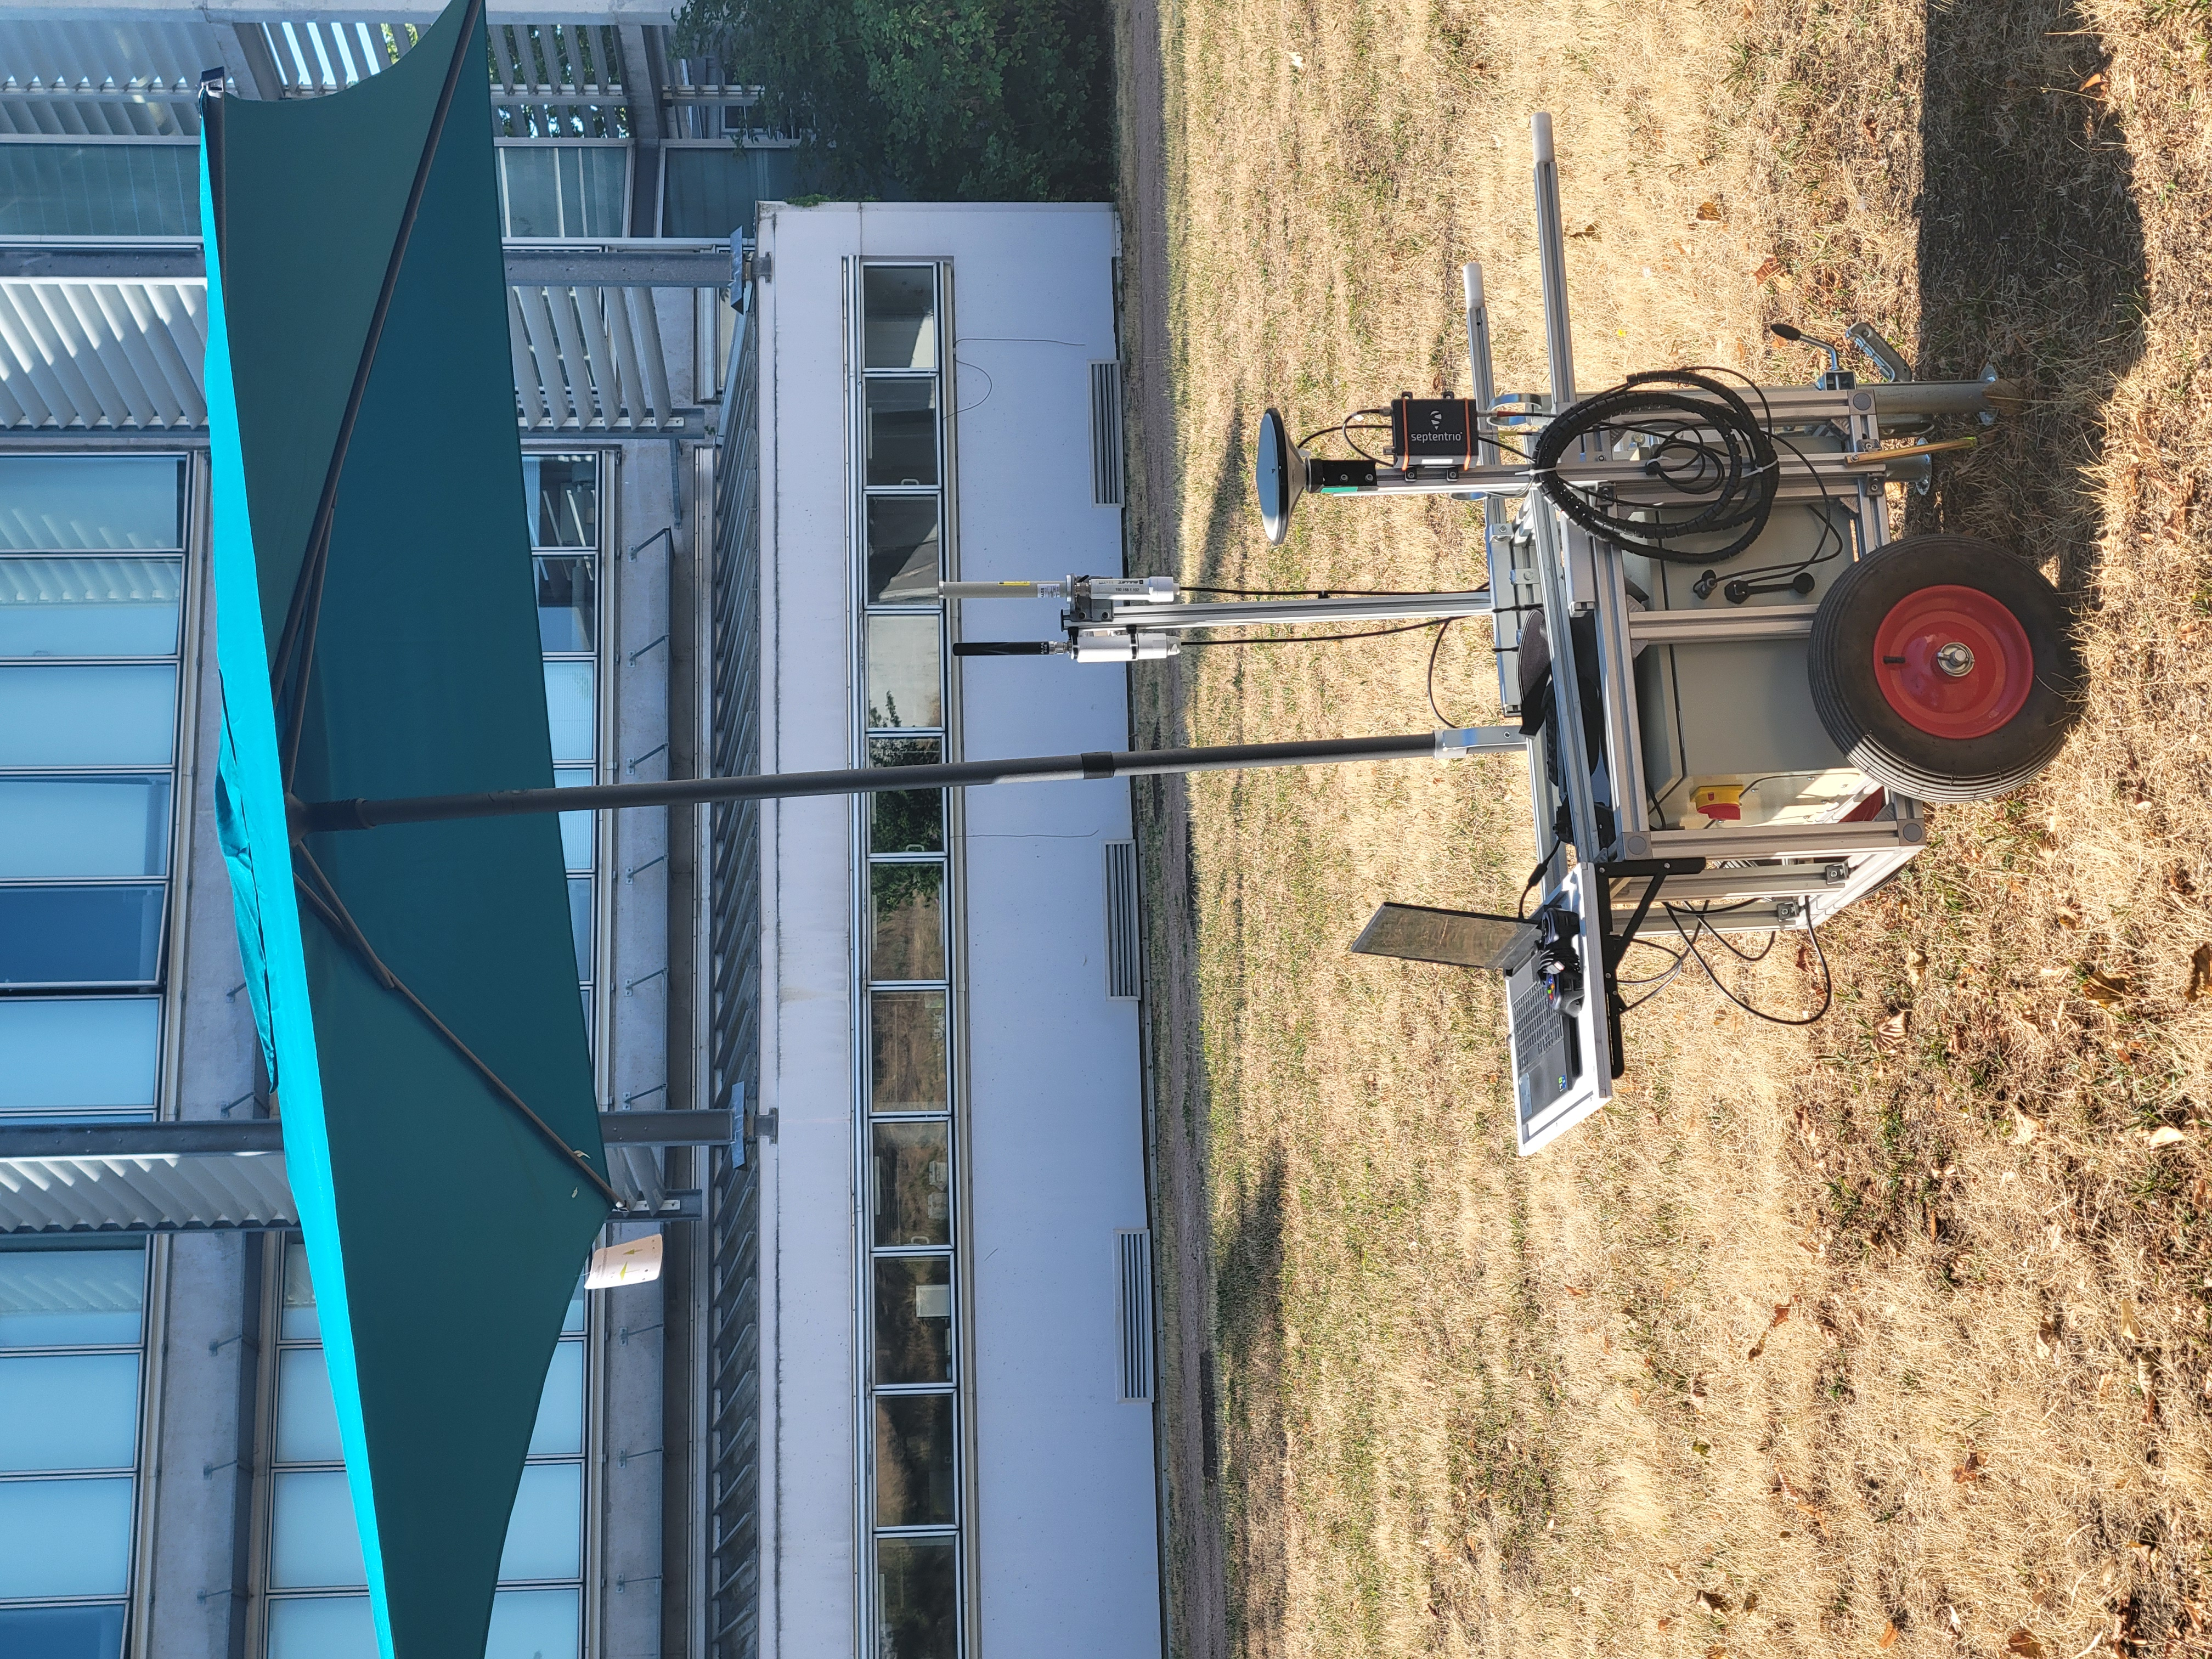
\includegraphics[width=0.5\linewidth, angle=-90]{Corps_rapport/PCC.jpg}
  \caption{Poste de Contrôle-Commande (PCC) débarqué}
  \label{fig10}
\end{figure}

L'ensemble de ces sous-systèmes s'articule selon l'architecture matérielle globale présentée sur la Figure~\ref{fig11} :

\begin{figure}[H]
  \centering
  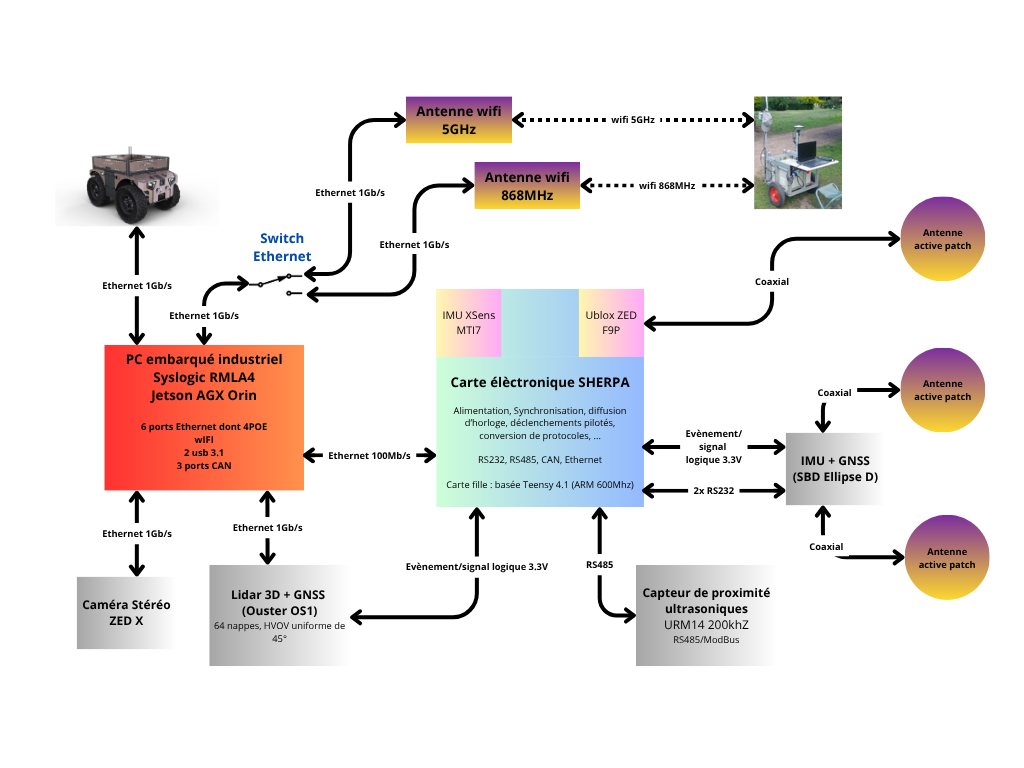
\includegraphics[trim={0.0cm 2cm 0.0cm 2cm}, clip, width=1\linewidth]{Corps_rapport/Architecture_système.png}
  \caption{Diagramme synoptique de l'architecture matérielle embarquée}
  \label{fig11}
\end{figure}

\subsection{Environnement de simulation Gazebo}
Afin de sécuriser les phases de développement et conformément aux méthodologies de validation logicielle en boucle ouverte/fermée, SHERPA Engineering a conçu un environnement de simulation sous Gazebo (Figure~\ref{fig12}). Ce jumeau numérique réplique fidèlement les interfaces d'entrées/sorties du robot ainsi que l'ensemble des flux capteurs (cf. graphe RQT en annexe~\hyperref[annexe1]{[I]}).\\\\
\indent Cette étape de simulation permet de valider le comportement des briques haut niveau (perception, cartographie, planification A* / DWA et génération de commandes) avant les essais sur plateforme réelle. L'environnement virtuel intègre des reliefs complexes, de la végétation et divers obstacles représentatifs des cahiers des charges de la DGA, et évolue au rythme des exigences des différents défis du challenge.

\begin{figure}[H]
  \centering
  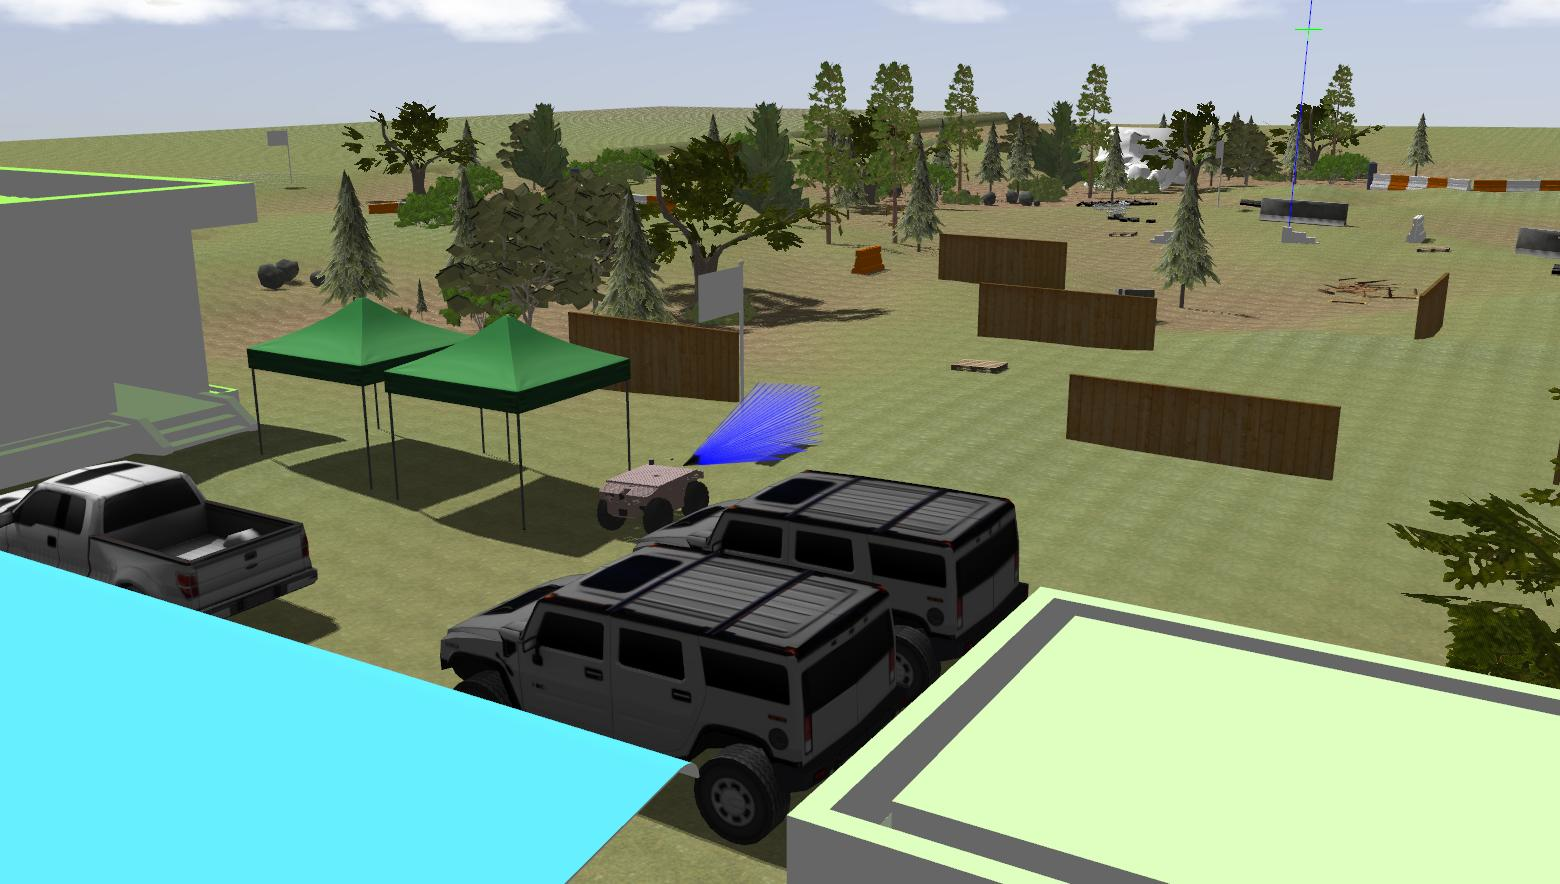
\includegraphics[width=1\linewidth]{Corps_rapport/gazebo_sim.png}
  \caption{Vue de l'environnement de simulation développé sous Gazebo}
  \label{fig12}
\end{figure}
